\documentclass[12pt,a4paper]{article}
\usepackage{amsmath,amscd,amsbsy,amssymb,latexsym,url,bm,amsthm}
\usepackage{epsfig,graphicx,subfigure}
\usepackage{enumitem,balance}
\usepackage{wrapfig}
\usepackage{mathrsfs,euscript}
\usepackage[usenames]{xcolor}
\usepackage{hyperref}
\usepackage{amsmath}
\usepackage[vlined,ruled,linesnumbered]{algorithm2e}
\hypersetup{colorlinks=true,linkcolor=black}

\newtheorem{theorem}{Theorem}
\newtheorem{lemma}[theorem]{Lemma}
\newtheorem{proposition}[theorem]{Proposition}
\newtheorem{corollary}[theorem]{Corollary}
\newtheorem{exercise}{Exercise}
\newtheorem*{solution}{Solution}
\newtheorem{definition}{Definition}
\theoremstyle{definition}

\renewcommand{\thefootnote}{\fnsymbol{footnote}}

\newcommand{\postscript}[2]
 {\setlength{\epsfxsize}{#2\hsize}
  \centerline{\epsfbox{#1}}}

\renewcommand{\baselinestretch}{1.0}

\setlength{\oddsidemargin}{-0.365in}
\setlength{\evensidemargin}{-0.365in}
\setlength{\topmargin}{-0.3in}
\setlength{\headheight}{0in}
\setlength{\headsep}{0in}
\setlength{\textheight}{10.1in}
\setlength{\textwidth}{7in}
\makeatletter \renewenvironment{proof}[1][Proof] {\par\pushQED{\qed}\normalfont\topsep6\p@\@plus6\p@\relax\trivlist\item[\hskip\labelsep\bfseries#1\@addpunct{.}]\ignorespaces}{\popQED\endtrivlist\@endpefalse} \makeatother
\makeatletter
\renewenvironment{solution}[1][Solution] {\par\pushQED{\qed}\normalfont\topsep6\p@\@plus6\p@\relax\trivlist\item[\hskip\labelsep\bfseries#1\@addpunct{.}]\ignorespaces}{\popQED\endtrivlist\@endpefalse} \makeatother

\begin{document}
\noindent

%========================================================================
\noindent\framebox[\linewidth]{\shortstack[c]{
\Large{\textbf{Lab02-Divide and Conquer}}\vspace{1mm}\\
CS214-Algorithm and Complexity, Xiaofeng Gao, Spring 2019.}}
\begin{center}
\footnotesize{\color{red}$*$ If there is any problem, please contact TA Jiahao Fan.}

% Please write down your name, student id and email.
\footnotesize{\color{blue}$*$ Name:KylinChen  \quad Student ID:517030910155 \quad Email: k1017856853@icloud.com}
\end{center}

\begin{enumerate}
    \item
    Consider the following recurrence:
    \begin{equation*}
    T(n)=
    \begin{cases}
    \ 0 & \text{if } n=1 \\
    \ 2T(n/2)+O(n\log{n}) & \text{if } n=2^k \text{ and } k \geq 1 \\
    \end{cases}
    \end{equation*}
    \begin{enumerate}
        \item
        Solve $T(n)$ (in the form of $O$-notation) by recurrence tree. Detailed derivation is required.
        \begin{solution}
        \renewcommand{\qedsymbol}{}
            In this part, we will first solve T(n) by recurrence tree, an then try to test and verify our 
            conclusion by recursive equation.\item
            \begin{itemize}
            \item
            \textbf{Analysis:} For this question, we can devide the original problem several times until each subproblem just costs T(1). \par
            Therefore, we can draw this recurrence tree Fig.~\ref{Recurrence}. In this picture, we can clearly see that every node(except root node) have the half scale of its father node, then we sum up all the O-notation values to get the T(n)'s O-notation.
            \begin{figure}[htbp]
            \centering
            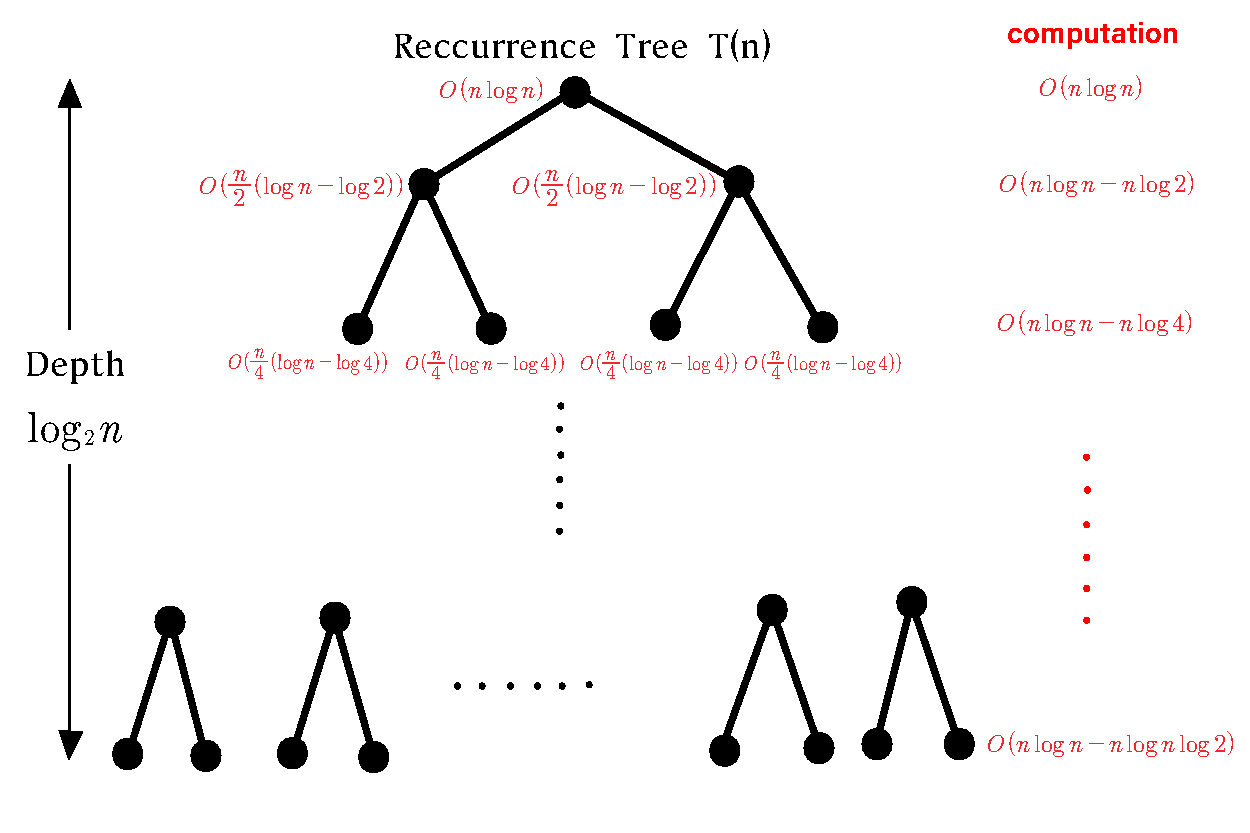
\includegraphics[width=0.8\textwidth]{figures/1_1.pdf}
            \caption{Reccurrence Tree}\label{Recurrence}
            \end{figure}\item
            \textbf{Calculation:} (In order to simplify the calculation process, we ignore the O-notation except 
            final result)
            $$T(n)=nlog(n)+n(log(n)-log(2))+n(log(n)-log(4))+\cdots+n(log(n)-log(n)log(2))$$
            $$\Rightarrow T(n)=nlog(n)log(n)-n(log(2)+2log(2)+3log(2)+...+log(n)lg(2))$$
            $$\Rightarrow T(n)=nlog(n)log(n)-nlog(2)\times \frac{((1+log(n))log(n))}{2}=n\cdot log(n)\times log(n)$$
            It means, in O-notation, $T(n)=O(n \cdot log^2(n))$.
            \item \textbf{Recursive Proof:} 
            Now we know, if $n=2^k\ and \ k\geq 1$, $T(n)=2T(\frac{n}{2})+O(nlogn)$, in order to simplify this recurrence, we substitute O(nlogn) to $\Theta(nlog_2n)$, it means T(n)=2T($\frac{n}{2}$)+$nlog_2n$, it's obvious if we get the $\Theta$-notation, in that way, it must be $O-notation$, too.\par
            We assume $n=2^m$, in which $m\geq 1$ Then we can make a substitution
            $$T(2^m)=2T(2^{m-1})+2^mlog_2(2^m)=2T(2^{m-1})+m\cdot 2^m$$
            Then, we define $f(m)=T(2^m)$, we get that
            \begin{align*}  
            f(m) &=  2f(m-1)+m\cdot 2^m 
            \\   &=  2(2\cdot f(m-2)+(m-1)\cdot2^{m-1})+m\cdot 2
            ^m
            \\   &=  4(2\cdot f(m-3)+(m-2)\cdot2^{m-2})+(m-1)\cdot 2^m + m \cdot 2^m
            \\   &=  8f(m-3)+(m-2)\cdot 2^m + (m-1)\cdot 2^m + m \cdot 2^m
            \\   &= \cdots \cdots
            \end{align*}
            In proceeding iteration, we can get that
            \begin{align*}  
            f(m) &=  2^m\cdot f(0)+2^m\cdot (1+2+3+4+5+\cdots+(m-1) +m)
            \\   &=  2^m\cdot f(0)+m\cdot (m+1)\cdot 2^{m-1}
            \\   &=  2^m\cdot f(0)+m(m-1)2^{m-1}
            \end{align*}
            Therefore, $T(n)=nT(1)+n(\frac{log_2(n)(1+log_2(n))}{2})=\Theta(n\cdot log^2n)$
            It means in O-notation, T(n)=$O(n\cdot log^2n)$, the recurrence tree get the correct result.
            \end{itemize}
        \end{solution}

        \item
        Can we use the Master Theorem to solve this recurrence? Please explain your answer.
        \begin{solution}
        \renewcommand{\qedsymbol}{}
            From my perspective, this recurrence can't use Master Theorem to solve, reasons can be summed up as follows: 
            \item
            \begin{itemize}
            \item For the recurrence $T(n)=2T(\frac{n}{2})+nlogn$, $a=2,b=2,f(n)=nlogn,and\ n^{log_b(a)}=n$\par
            In this case, f(n) is asymptotically larger than $n^{log_b(a)}$, but not polynomially larger. Thus, Master Theorem doesn't apply here.
            \item In wikipedia Master theorem (analysis of algorithms), we can find a $\varepsilon$-definition, for this question, the ratio $logn$ is asymptotically less than $n^{\varepsilon}$ for any positive $\varepsilon$.
            \item In the recursive proof in part(a), we can find this this solving process is totally like Master Theorem's derivation. And if we use Master Theorem in this question, it can get correct answer.
            So, it may use \textbf{General Master Theorem}, which can refers to MIT edition.
            \end{itemize}
            
        \end{solution}

    \end{enumerate}

    \item
    Given any array $num$, find the number of pairs $(i, j)$ satisfying $i < j$ and $num[i] > 2 \times num[j]$. For example, if $num=[1,3,2,3,1]$, the answer should be 2.
    \begin{enumerate}
        \item
         Design an algorithm to solve this problem using divide-and-conquer strategy and complete the implementation in the provided C/C++ source code. {\color{blue}(The source code \emph{Code-Pairs.cpp} is attached on the course webpage.)}\par
         {\color{red}(.cpp file is attached to the compress file)}

        \item
        Write a recurrence for the running time of your algorithm and solve it using the Master Theorem directly.
        \begin{solution}\item
        \renewcommand{\qedsymbol}{}
            \begin{itemize}
            \item [(a)] This algorithm relies on \textbf{MergeSort Algorithm}, which can be achieved by private function(refers to .cpp file) PairsCount. Its idea can be summed up as follows:
                \begin{itemize}
                \item According to \textbf{DevideAndConquer}, if the input array's size is more than one, we can devide it into sub-array A and sub-array B, which refers to Fig.~\ref{Array}
                \item 
                Then we recursively calling the function PairCount to accumulate the number of aimed-pair.
                In this process, we use mergesort to sort this array, ao that we can get $O(n)$ complexity every count step.
                \item 
                For accumulate the aimed-pair, we just do it between sub-array A and B. And if a1$\geq$b2, we can directly claim a2$\geq$b2 because array A is a nondecreasing array, therefore we just get linear time-complexity every recurrence.
                \end{itemize}
                Repeat these steps until recursive termination, we can get the returning value count for correct answer.
                \begin{figure}[htbp]
                \centering
                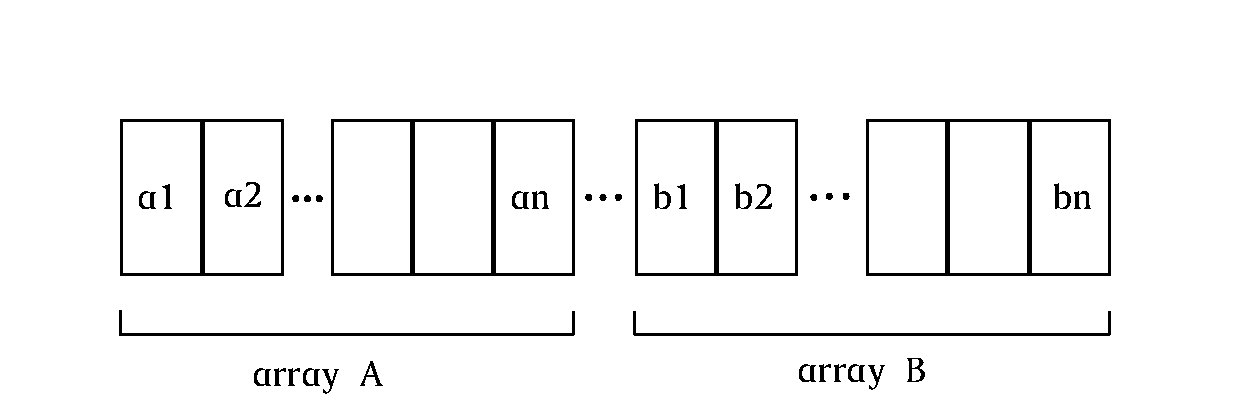
\includegraphics[width=0.8\textwidth]{figures/1_2.pdf}
                \caption{Devide one array into two subarrays}\label{Array}
                \end{figure}
                
            \item [(b)] According to algorithm subscription in (a), we can make an analysis:
            \begin{itemize}
            \item In each step we divide the array into 2 sub-arrays, and hence, every sub-array takes $\frac{n}{2}$ problem size.
            \item Additional $O(n)$ work needs to be done to count the inversions and to merge the 2 sub-arrays after sorting. 
            \end{itemize}
            Therefore, we can get recurrence:
            $$T(n)=2T(\frac{n}{2})+O(n)$$
            By \textbf{Master Theorem}, $log_ba=1=d$, so the running time T(n)=O(nlog(n)). 
            \end{itemize}
        \end{solution}
    \end{enumerate}

    \item
    \textbf{Transposition Sorting Network}: A comparison network is a \textbf{transposition network}  if each comparator connects adjacent lines, as in the network in Fig.~\ref{Fig-Transposition}.

    
    
    \begin{enumerate}
        \item
        Prove that a transposition network with $n$ inputs is a sorting network if and only if it sorts the sequence $\langle n, n-1, \cdots, 1 \rangle$. {\color{blue}(Hint: Use an induction argument analogous to the \emph{Domain Conversion Lemma}.)}
        \begin{proof}\textbf{1}\item
        \renewcommand{\qedsymbol}{}
           \begin{itemize}
            \item First, we will prove that if a comparator(two line sorting network) can correct sort number pair (for example $<1,2>$, $<2,3>$, $<3,4>$ $\cdots$ $<n-1,n>$) it can sort any other number pair.\par
            For the comparator in Fig.~\ref{Comparator}. When inputs is \{x,y\}, the upper output must be min\{x,y\} while lower is max\{x,y\}.\par
            Then we can find a linear function f(x), which is monotonically increasing. Consequently we have the identity:
            $$min\{f(x),f(y)\} = f(min\{x,y\})$$
            $$max\{f(x),f(y)\} = f(max\{x,y\})$$
            Thus, we can make a linear conversion from \{x,y\} to aimed \{f(x),f(y)\}, it is also correctly sorted. 
            \begin{figure}[htbp]
             \centering
            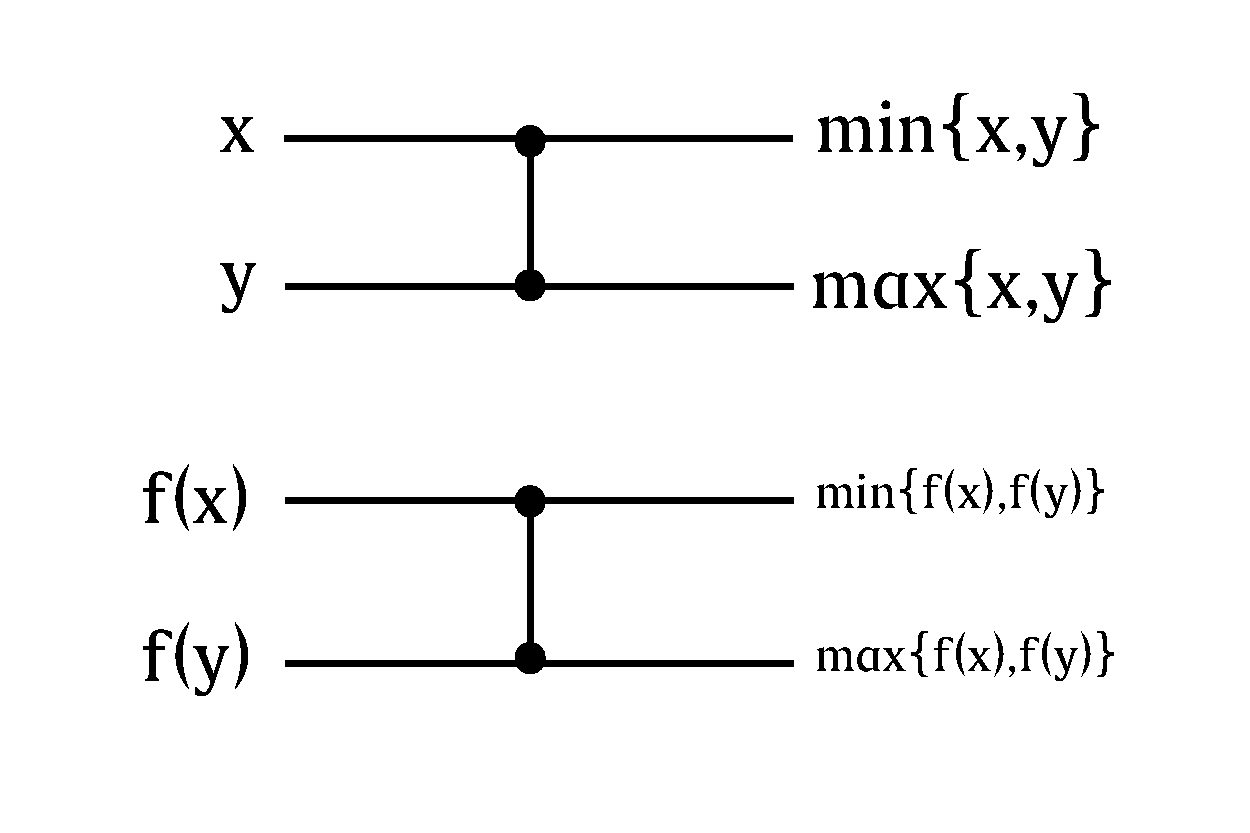
\includegraphics[width=0.4\textwidth]{figures/1_3.pdf}
            \caption{Comparator(Two-line Sorting Network)}\label{Comparator}
            \end{figure}
            \item If we assume k-1 line transposition network is sorting network (k-1 values are correctly sorted using previous comparators), then we want to prove k line transposition network is sorting network.\par
            Once we attach k-th line to k-1 network, it must be added by the sides, otherwise it can attribute to previous already-proved condition.\par
            From Fig.~\ref{Induction} We can obviously get that once k-th line is added, we will add n-1 comparators.\par
            Since,$$n_{(comparators)}=n-1=n_{(beforeArray)}\geq Move-Step_{max}$$ 
            Therefore, we can claim k values are well sorted and k line transposition network is sorting network.
            \begin{figure}[htbp]
             \centering
            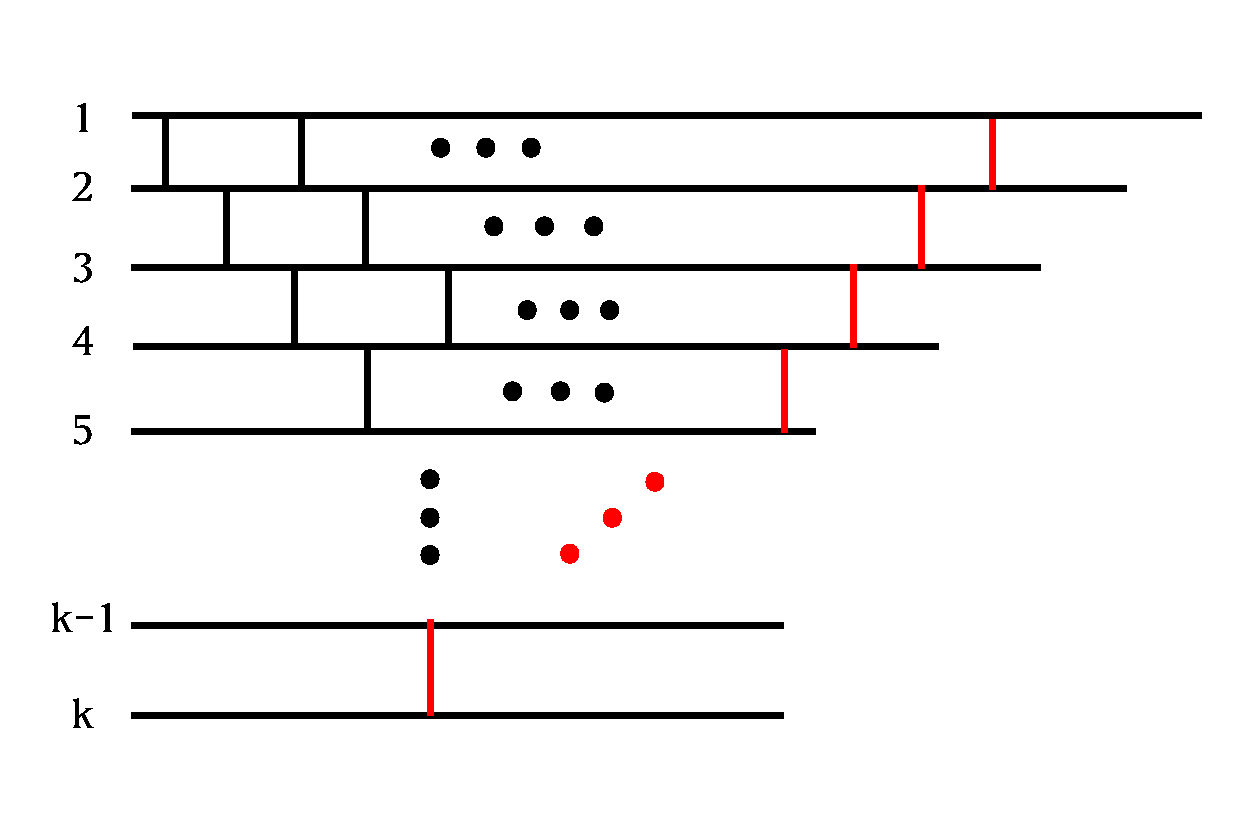
\includegraphics[width=0.5\textwidth]{figures/1_4.pdf}
            \caption{Induction from k-1 to k}\label{Induction}
            \end{figure}
           \end{itemize}
           According to mathmatical induction, we can claim if and only if a transposition network sorts the sequence $(n,n-1,\cdots,1)$, it is a sorting network.
        \end{proof}
        \begin{proof}\textbf{2}\item
        \renewcommand{\qedsymbol}{}
        We can change original proposition's expression as follows:\item
        For a data sequence $X={x_1,x_2,x_3,\cdots,x_n}$, we use symbol $i_{X,k}$ to express the data on i-th line after going through k-th comparator.\item
        \textbf{Equivalent proposition:} For data sequence $D=(n,n-1,n-2,\cdots,1)$ and arbitrary sequence $X=(x_1,x_2,x_3,\cdots,x_n)$, with the final L-th comparator and $i<j$, 
        $i_{D,L}<j_{D,L}$ if and only if $i_{X,L}<j_{X,L}$.\item
        We use induction to prove the equivalent proposition, so we assume: for r lines in this transposition network, after going through k-th comparator, for any $1\leq i \leq j \leq r$, $i_{D,k} \leq j_{D,k}$. (Our aim is to derive $i_{X,k} \leq j_{X,k}$) 
        \begin{itemize}
        \item If $|i-j|=1$, no matter whether i,j is the last reverse pair or not, comparator will sort it in increasing order, so it's obvious to get $i_{X,k} \leq j_{X,k}$.
        \item If $|i-j| \ne 1$, in this time, i and j are not connected by comparator, which means the data on these two line is kept, that is to say, $i_{X,k} = j_{X,k-1}$ and $i_{X,k} = j_{X,k-1}$. By induction assumption, we can get $i_{X,k-1} \leq j_{X,k-1}$, so $i_{X,k} \leq j_{X,k}$.
        \end{itemize}
        In summary, a transposition network with n inputs is a sorting network if and only if it sorts the sequence $D=(n,n-1,n-2,\cdots,1)$.
        \end{proof}

        \item
        {\color{red}{(Bonus)}} Given any $n \in \mathbb{N}$, write a program using Tkinter in Python to draw a figure similar to Fig.~\ref{Fig-Transposition} with $n$ input wires.
        \begin{figure}[htbp]
        \centering
        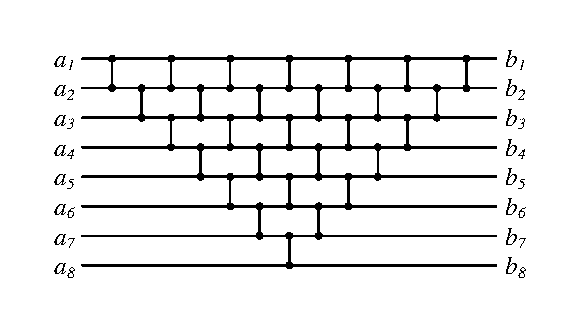
\includegraphics[width=0.5\textwidth]{figures/Fig-Transposition.pdf}
        \caption{A Transposition Network Example}\label{Fig-Transposition}
        \end{figure}
        \begin{solution}
        \renewcommand{\qedsymbol}{}
        {\color{blue}The attached file \textbf{transposition.py} is submission python code.}\item
        Require python package Tkinter.\item Test pass with PyCharm, Anaconda 3.7 version, macOS.
        \begin{figure}[htbp]
        \centering
        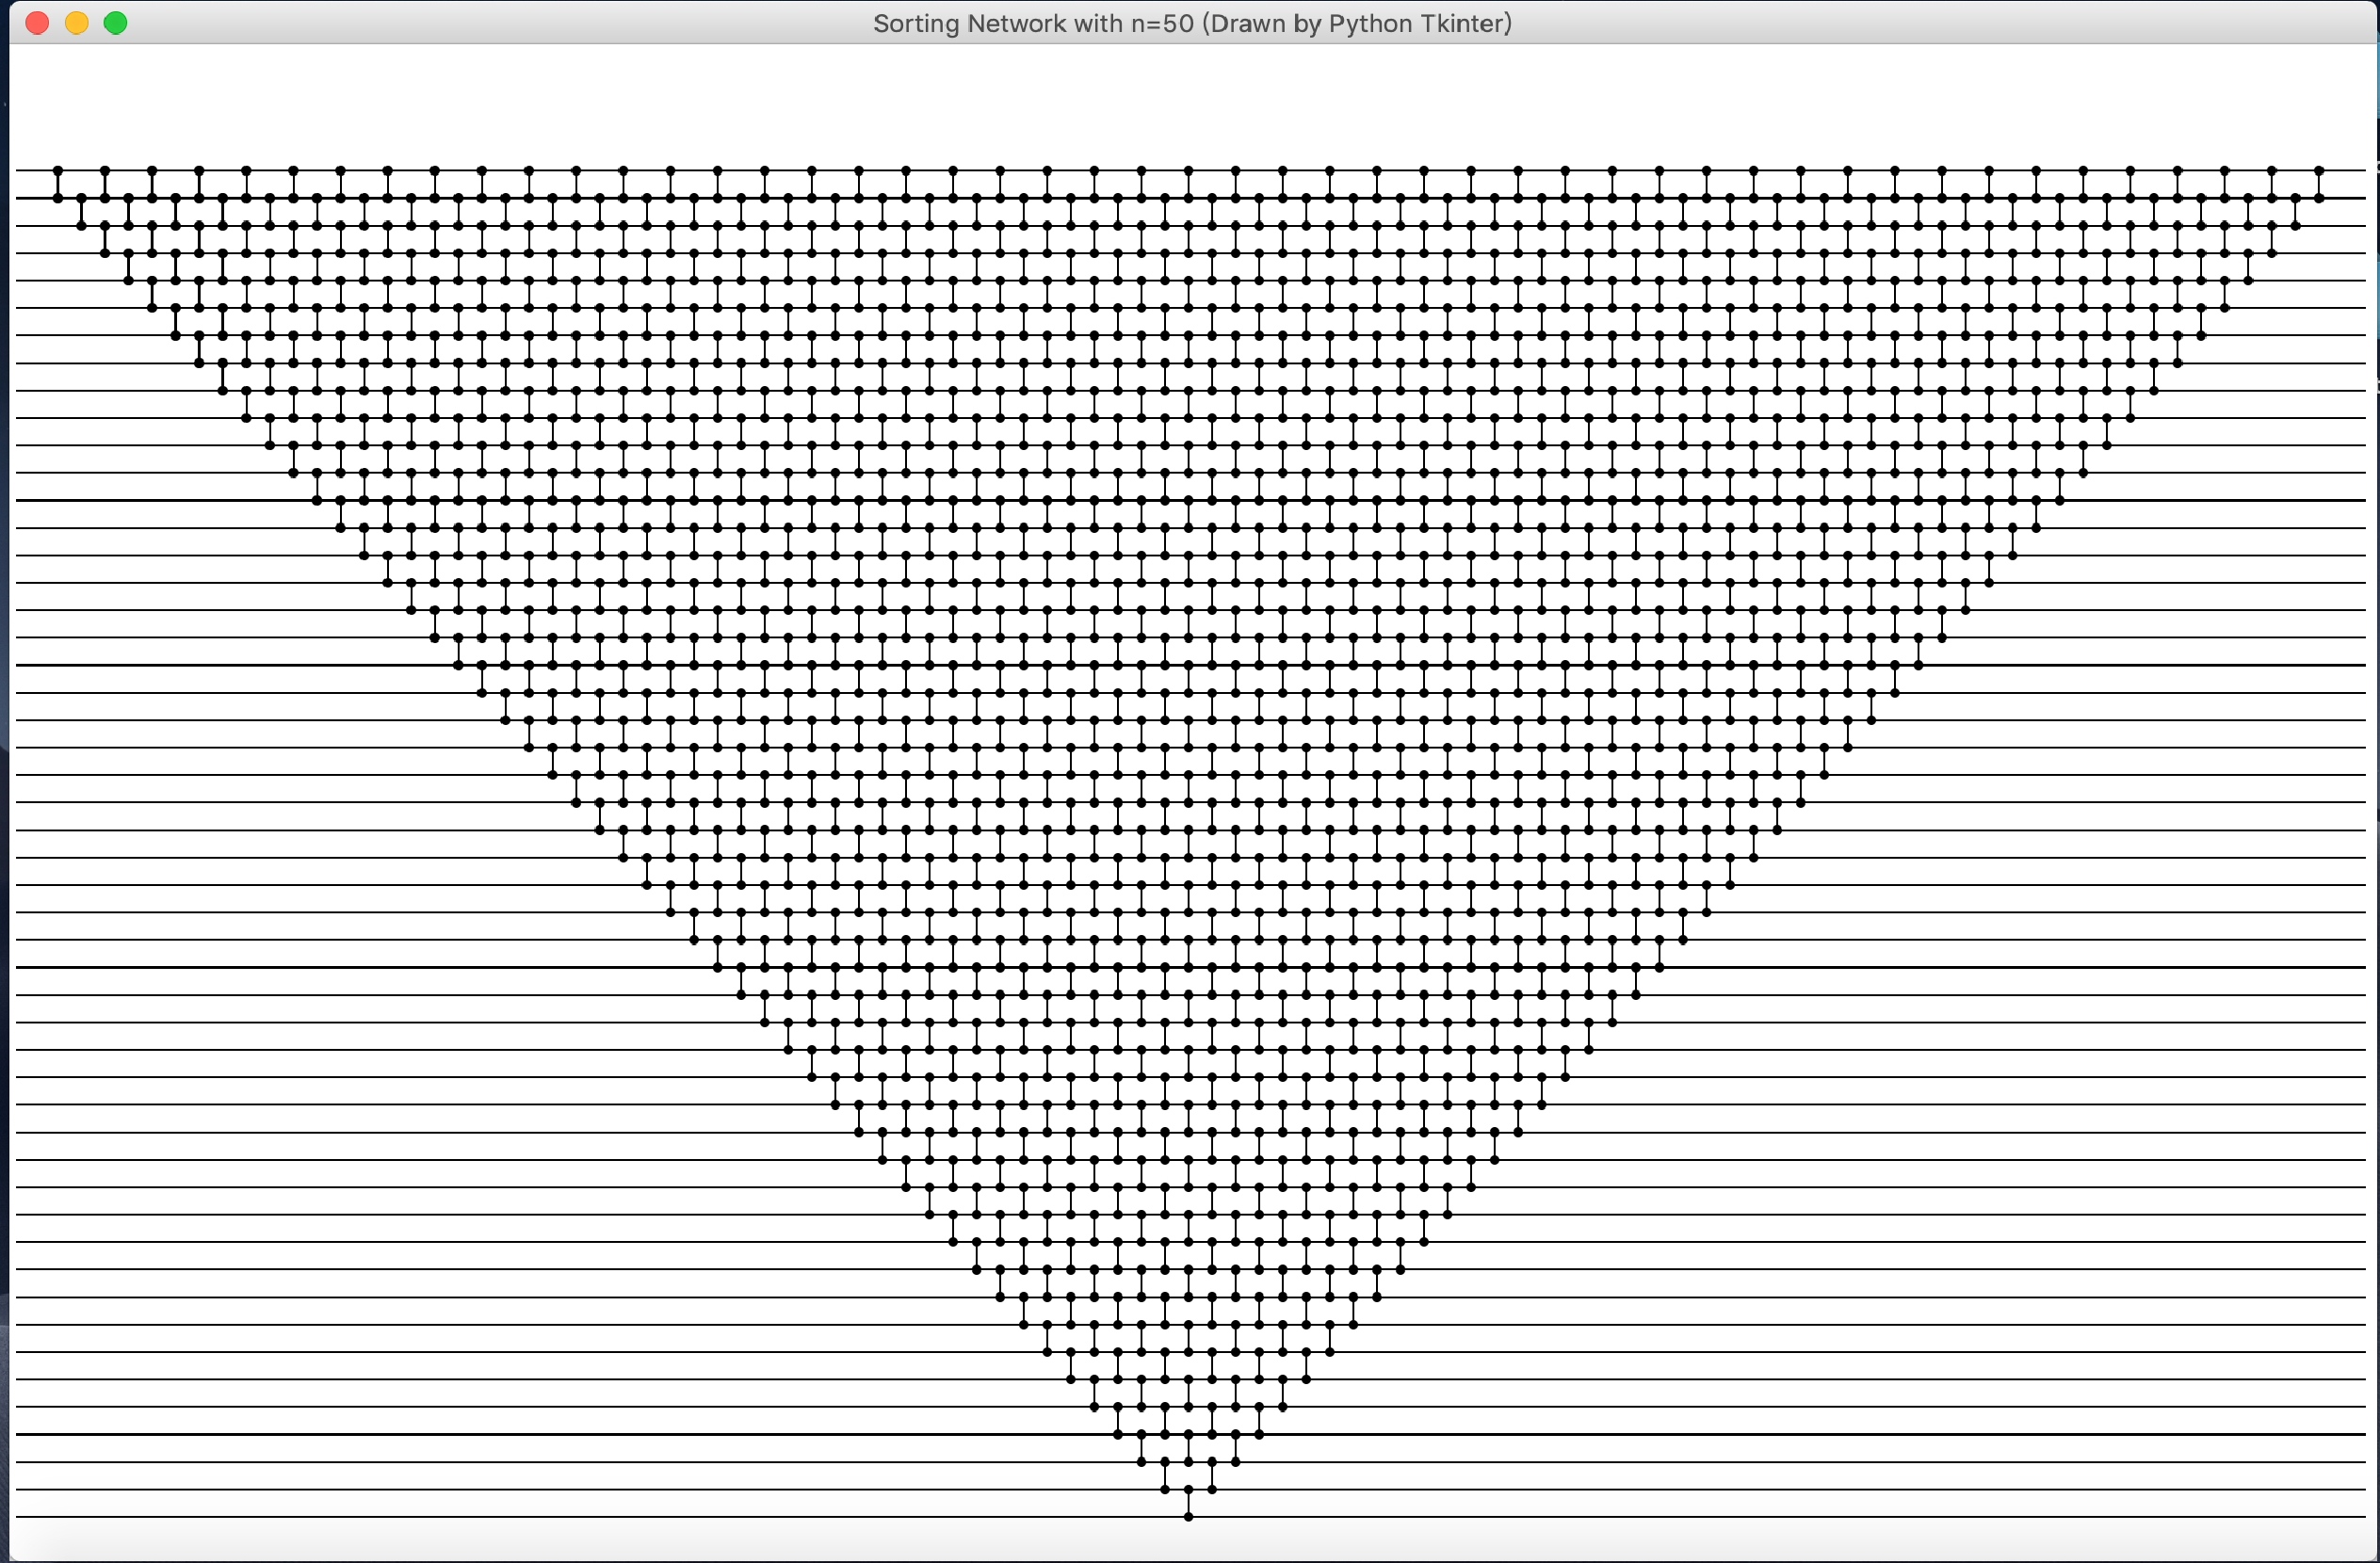
\includegraphics[width=0.8\textwidth]{figures/1_5.pdf}
        \caption{\textbf{transposition.py} Test with n=50}\label{Test}
        \end{figure}
        \end{solution}
    \end{enumerate}

\end{enumerate}

\vspace{20pt}

\textbf{Remark:} include your .cpp, .py, .pdf and .tex files in your uploaded .rar or .zip file.

%========================================================================
\end{document}
